\documentclass[11pt]{article}

%% Page geometry
\usepackage[a4paper, margin=1in]{geometry}

%% Core math + fonts
\usepackage{amsthm,amsmath,amsfonts,amssymb}
\usepackage{lmodern}
\usepackage{microtype}

%% Citations
\usepackage[authoryear, round]{natbib}

%% Colour (for revision marks)
\usepackage{xcolor}

%% Hyperlinks
\usepackage[colorlinks, citecolor=blue, urlcolor=blue, linkcolor=blue]{hyperref}
\usepackage{xurl}

%% Graphics & figures
\usepackage{graphicx}
\graphicspath{{figures/}{./figures/}}
\usepackage{float}
\usepackage{subcaption}
\usepackage{booktabs}

%% Float placement: every float carries [!tb], so figures and tables sit at
%% the top or the bottom of a page and never on a page of their own. The
%% fractions below widen the top and bottom areas so a float rarely has to be
%% deferred, and floatpagefraction is set high so that a float page would have
%% to be nearly full to be worth making.
\renewcommand{\topfraction}{0.9}
\renewcommand{\bottomfraction}{0.9}
\renewcommand{\textfraction}{0.07}
\renewcommand{\floatpagefraction}{0.9}
\setcounter{topnumber}{3}
\setcounter{totalnumber}{4}
\usepackage[section]{placeins}  % keep floats within their section

%% Algorithms
\usepackage[linesnumbered, ruled, vlined]{algorithm2e}

%% TikZ for diagrams
\usepackage{tikz}
\usetikzlibrary{shapes,arrows,fit,calc,positioning}
\tikzset{box/.style={draw, diamond, thick, text centered, minimum height=0.5cm, minimum width=1cm}}
\tikzset{line/.style={draw, thick, -latex'}}

%% Misc
\usepackage{comment}
\usepackage{dsfont}
\usepackage{enumitem}
\usepackage{changepage}
\usepackage{bm}

%% Theorem environments
\theoremstyle{plain}
\newtheorem{axiom}{Axiom}
\newtheorem{claim}[axiom]{Claim}
\newtheorem{theorem}{Theorem}[section]
\newtheorem{lemma}[theorem]{Lemma}
\newtheorem{assumption}{Assumption}
\newtheorem{proposition}{Proposition}
\newtheorem{corollary}{Corollary}

\theoremstyle{definition}
\newtheorem{definition}[theorem]{Definition}
\newtheorem*{example}{Example}
\newtheorem*{fact}{Fact}

\theoremstyle{remark}
\newtheorem{case}{Case}
\newtheorem{remark}{Remark}

%% Biostatistics prints the abstract under the heading "Summary".
\renewcommand{\abstractname}{Summary}

%% Custom math commands
\newcommand{\E}{\mathbb{E}}
\newcommand{\1}{\mathds{1}}
\newcommand{\p}{\mathbb{P}}
\renewcommand{\H}{\mathcal{H}}
\newcommand{\T}{\mathcal{T}}
\newcommand{\ind}{\perp\!\!\!\perp}
\newcommand{\RCT}{\mathrm{RCT}}
\newcommand{\RWD}{\mathrm{RWD}}
\newcommand{\AF}{\mathrm{AF}}
\newcommand{\expit}{\operatorname{expit}}


\title{Bayesian fusion forests for heterogeneous treatment effects on survival from randomised and real-world data}



%% Affiliations are set as a numbered block on the title page rather than
%% through \thanks: Biostatistics does not allow footnotes.
\author{
  Tijn Jacobs$^{1,\ast}$ \quad
  St\'ephanie L.\ van der Pas$^{1}$ \quad
  Wessel N.\ van Wieringen$^{1, 2}$
}

\date{}

\setlength{\parindent}{0pt}
\setlength{\parskip}{0.8em}


\begin{document}

%% --- Numbers of supplement (SM) objects, hardcoded so the main file is
%% self-contained (no sm.aux / xr-hyper). Update if the SM numbering changes.
\makeatletter
\@namedef{r@sm:proofs}{{S.1}{}{}{}{}}
\@namedef{r@sm:map-m0}{{S.2}{}{}{}{}}
\@namedef{r@sm:posterior-computation}{{S.3}{}{}{}{}}
\@namedef{r@sm:sim-additional}{{S.4}{}{}{}{}}
\@namedef{r@sm:analysis-additional}{{S.5}{}{}{}{}}
\@namedef{r@sm:analysis-competitors}{{S.5.2}{}{}{}{}}
\makeatother

\maketitle

%% --- Page-1 information required by Biostatistics. Two blocks rather than
%% one: who the authors are sits under the title, and the declarations are
%% pushed to the foot of the page by \vfill. Stacking all five against the
%% title left a dense block up top and an empty page below it. ---

\begin{center}
\begin{minipage}{0.9\textwidth}
\setlength{\parskip}{0.4em}
\small
\noindent
$^{1}$Department of Mathematics, Vrije Universiteit Amsterdam \\
$^{2}$Department of Epidemiology and Data Science, Amsterdam University Medical Centre

\noindent
$^{\ast}$Corresponding author: Tijn Jacobs, \texttt{t.jacobs@vu.nl}.
\end{minipage}
\end{center}


\begin{abstract}
We develop the \emph{Bayesian fusion forest}, a nonparametric framework to estimate heterogeneous treatment effects on survival outcomes by combining a randomised controlled trial and real-world data.
The framework relaxes the unconfoundedness assumption on the real-world data by assuming instead that the treatment effect transports across the two sources.
Our method opens up right- and interval-censored outcomes to data fusion.
We model the survival time with an accelerated failure time decomposition into a shared baseline prognosis, a source-specific deviation, a treatment effect, and a confounding function.
The confounding function absorbs the confounding bias in the real-world data.
Each component receives a Bayesian tree ensemble prior.
The shared baseline prognosis borrows strength across sources, while the deviation captures between-source heterogeneity.
A hierarchical Dirichlet process mixture models the error distribution nonparametrically.
A simulation study shows efficiency gains over a trial-only analysis across varying levels of confounding and between-source heterogeneity.
We combine the ACTG~175 trial with the Multicenter AIDS Cohort Study to estimate the effect of combination antiretroviral therapy for HIV.
The fusion identifies a benefit for nearly every patient whereas the trial alone is inconclusive.

\medskip
\noindent\textbf{Keywords:} Bayesian additive regression trees; data fusion; heterogeneous treatment effects; real-world evidence; survival analysis; unmeasured confounding.
\end{abstract}

\vfill

\begin{center}
\begin{minipage}{0.92\textwidth}
\footnotesize
\setlength{\parskip}{0.7em}
\rule{\linewidth}{0.4pt}

\noindent
\textbf{Funding.}
This work was supported by the European Research Council [grant number
101074802]; and the SURF Cooperative [grant number EINF-18803].
Views and opinions expressed are those of the authors only and do not
necessarily reflect those of the European Union or the European Research
Council Executive Agency.
Neither the European Union nor the granting authority can be held responsible
for them.

\noindent
\textbf{Acknowledgements.}
The authors used generative artificial intelligence tools in support of
developing and debugging the accompanying software.
All such output was reviewed and verified by the authors, who take full
responsibility for the content of this work.

\noindent
\textbf{Conflict of interest.}
None declared.
\end{minipage}
\end{center}


%% Keep the front matter to itself: no float may drift onto the title page or
%% the abstract page. The fractions above are deliberately permissive so that
%% floats sit beside text rather than on pages of their own, and without this
%% barrier that permissiveness reaches the front matter too.
\FloatBarrier

% !TEX root = ../general/main.tex
\section{Introduction}

Precision medicine uses heterogeneous treatment effects (HTE) to guide clinical decisions.
Researchers estimate the HTE from either a randomised controlled trial (RCT) or observational real-world data (RWD).
Randomised trials are the gold standard for causal effect estimation, but they are underpowered for subgroup effects and often have limited follow-up.
Real-world data from registries and cohorts are larger and often follow patients for longer.
Regulators increasingly accept them as evidence.
Unmeasured confounding can bias treatment effect estimates from observational data.
We combine the two data sources. We identify the effect from the trial and borrow power and longer follow-up from the real-world data.
Our motivating example is HIV antiretroviral therapy.
The treatment effect varies with baseline CD4 count, viral load, and age.
We fuse the ACTG~175 trial \citep{hammer1996} with the Multicenter AIDS Cohort Study \citep{kaslow1987}.
The cohort followed participants over more than 25 years with biannual visits.

The fusion of a trial with real-world data raises three challenges for survival outcomes.
The first is unmeasured confounding in the real-world data.
Treatment is not randomised, and assignment depends on factors the measured covariates do not fully capture.
The no-unmeasured-confounders assumption is untestable and often violated in practice \citep{vanderweele2017evalue}.
The second is heterogeneity between the two data sources.
Even when the treatment effect transports across sources, the baseline prognosis often does not.
The trial and observational populations typically differ in eligibility, follow-up, and case mix.
A naive analysis confounds this baseline difference with the treatment effect.
This heterogeneity is not confined to the mean: differences in measurement protocol and follow-up quality also reshape the error distribution across sources.
The third is the survival outcome.
Right censoring arises when the event has not occurred by the end of follow-up, so the survival time is known only to exceed the censoring time.
The real-world data may also be interval-censored, with events recorded only at periodic visits.

Unmeasured confounding can be addressed through a confounding function.
The confounding function measures the confounding bias in the real-world data.
It was introduced as a sensitivity-analysis device within a single study \citep{robins2000sensitivity}.
The confounding function can be estimated by combining a randomised and an observational study.
\citet{Kallus2018} learn the confounding function from the RCT and debias the observational treatment effect.
\citet{YangLiuZengWang2025} develop a semiparametric-efficient estimator that jointly estimates the treatment effect and the confounding function, and derive a test for unmeasured confounding.
The elastic integrative estimator of \citet{yang2023elastic} uses that test to decide whether to borrow from the real-world data, and discards it when confounding is detected.
Two frequentist methods extend the approach to survival outcomes.
\citet{Ye2025} work under an accelerated failure time model with right censoring and high-dimensional covariates, and treat the confounding function as a sparse component selected jointly with the treatment effect.
\citet{mao2025statistical} target the conditional restricted mean survival time under right censoring.


Bayesian methods combine data sources by borrowing information through the prior.
The power prior of \citet{ibrahim2000power} raises the external likelihood to a fractional power that controls the borrowing.
The meta-analytic-predictive prior of \citet{neuenschwander2010} makes the borrowing hierarchical and adaptive to between-source heterogeneity.
Later variants tie the borrowing to the between-source discrepancy through commensurate priors \citep{hobbs2012commensurate}.
These methods all target a marginal or control-arm effect.
More recent literature targets heterogeneous effects directly.
\citet{zhou2021incorporating} pool trial and external outcome surfaces with Bayesian additive regression trees, but do not allow for unmeasured confounding in the external source.
\citet{dimitriou2025causal} develop a multi-task Gaussian process with a data-adaptive borrowing parameter.
None of these Bayesian methods targets heterogeneous treatment effects on survival outcomes under unmeasured confounding.

Bayesian additive regression trees \citep{chipman2010bart} are a popular method for causal machine learning \citep{hill2011bayesian}.
They are supported by theoretical guarantees \citep{rockova2020posterior} and have strong empirical performance in both estimation accuracy and uncertainty quantification \citep{dorie2019, thal2023, kabata2026}.
The uncertainty quantification is intrinsic to the model and follows directly from the posterior distribution.
Black-box predictors such as (deep) neural networks are flexible alternatives, but do not provide intrinsic uncertainty quantification and do not separate the causal effect from confounding bias.
We will show that a structured approach tailored to the problem at hand and its statistical constraints outperforms a generic black-box competitor in both accuracy and calibration.

We develop a Bayesian nonparametric framework to estimate heterogeneous treatment effects on survival outcomes.
We target the acceleration factor, a causally interpretable estimand on the survival-time scale.
We fuse a randomised trial with real-world data without assuming the observational source is unconfounded.
A confounding function absorbs the bias from unmeasured confounding in the real-world data.
We accommodate right- and interval-censored data, and exploit the longer follow-up of the real-world source for robustness.
A hierarchical Dirichlet process mixture models the error distribution nonparametrically and lets it vary across sources.

% !TEX root = ../general/main.tex
\section{Methodology}

\subsection{Causal framework}

We consider data from two sources: a randomised controlled trial (RCT) and a real-world data study (RWD).
The data-source indicator $S \in \{0, 1\}$ takes the value $S = 1$ for RCT observations and $S = 0$ for RWD observations.
The RCT contributes $n_1$ independent observations and the RWD contributes $n_0$ independent observations.
We observe a vector of pre-treatment covariates $X \in \mathbb{R}^p$ and a binary treatment $A \in \{0, 1\}$ for each individual.
The outcome of interest is the nonnegative survival time $T$, subject to censoring.
We allow two types of censoring: right censoring, and interval censoring.
For each subject we observe a pair $(L, R)$ with $0 \leq L \leq R \leq \infty$ satisfying $T \in [L, R]$, together with a censoring-type indicator $\delta \in \{0, 1, 2\}$.
We use the convention that $R = \infty$ stands for $T \in [L, \infty)$.
These correspond to exact observation ($\delta = 1$: $L = R = T$), right censoring ($\delta = 0$: $L = C$ and $R = \infty$, for some censoring time $C$), and interval censoring ($\delta = 2$: $0 \leq L < R < \infty$).
The standard right-censored setup is recovered when $\delta \in \{0, 1\}$ for every subject.
We write $\mathcal{C}$ for the inspection and censoring process underlying $(L, R, \delta)$, and refer to \citet{sun2006statistical} for background.
We adopt the potential-outcomes framework \citep{rubin1974}: $T(a)$, $\mathcal{C}(a)$, and the corresponding observations $(L(a), R(a), \delta(a))$ are defined analogously under treatment $A = a$.


We estimate the conditional average treatment effect (CATE):
\begin{equation}
\tau(x) = \E[\log T(1) - \log T(0) \mid X = x].
\label{eq:cate}
\end{equation}
The CATE captures the heterogeneity of the treatment effect across covariate values.
The corresponding estimand on the multiplicative time scale is the acceleration factor $\exp\{\tau(x)\}$.
The acceleration factor admits a direct interpretation on the survival-time scale: at every quantile of the survival distribution, treatment rescales the survival time by a constant multiplicative factor \citep{Brathovde2024}.
This time-scaling is more intuitive in a clinical setting than the relative change in event rate conveyed by a hazard ratio \citep{Swindell2009}.
The acceleration factor also enjoys causal properties that the hazard ratio lacks.
\citet{Brathovde2024} show that the observed acceleration factor identifies its causal counterpart under exchangeability and consistency.
This identification continues to hold under unmeasured frailty and treatment-effect heterogeneity.
The hazard ratio loses its causal interpretation in those same settings, because conditioning on survival induces a built-in selection bias \citep{hernan2010}.
The acceleration factor is collapsible: the marginal and conditional acceleration factors coincide when the treatment effect is homogeneous, regardless of the distribution of unmeasured baseline risk \citep{Aalen2015, Crowther2023}.

We impose conditions on the causal structure of the problem and on the censoring mechanism.
\vspace*{-\parskip}
\begin{adjustwidth}{1.5em}{1.5em}
\setlength{\parskip}{0pt}
\begin{assumption}[Consistency]\label{ass:sutva}
$T = A\,T(1) + (1 - A)\,T(0)$.
\end{assumption}

\begin{assumption}[Unconfoundedness of the RCT]\label{ass:rct-unconf}
$T(a) \,\ind\, A \mid X,\, S = 1$ for each $a\in\{0, 1\}$.
\end{assumption}

\begin{assumption}[Positivity]\label{ass:positivity-both}
$0 < \p(A = 1 \mid X = x,\, S = s) < 1$ for each $s \in \{0, 1\}$ and all $x$ in the support of $X \mid S = s$.
\end{assumption}

\begin{assumption}[Cross-source exchangeability]\label{ass:transport}
$T(a) \mid X,\, S = 1 \;\overset{d}{=}\; T(a) \mid X,\, S = 0$, for each $a \in \{0, 1\}$.
\end{assumption}

\begin{assumption}[Conditionally non-informative censoring]\label{ass:censoring}
$T(a) \,\ind\, \mathcal{C}(a) \mid X,\, A,\, S$ for each  $a\in\{0, 1\}$.
\end{assumption}

\end{adjustwidth}
\setlength{\parskip}{0.8em}
\vspace{0.8em}


\begin{remark}[Possible weakening to CATE-only transport]
Assumption~\ref{ass:transport} may be stronger than needed.
It could be replaced by the weaker condition that only the conditional log-treatment effect transports across sources:
\begin{equation}
\E[\log T(1) - \log T(0) \mid X,\, S = 1] \;=\; \E[\log T(1) - \log T(0) \mid X,\, S = 0].
\label{eq:cate-transport}
\end{equation}
This alleviation may suffice in our setting because the causal estimand is the CATE on the log-time scale.
\textit{To be verified.}
\end{remark}


Our identification strategy relaxes unconfoundedness in the RWD and retains transportability of the CATE across sources.
Assumption~\ref{ass:rct-unconf} holds by design in a randomised trial.
Treatment in the RWD may depend on confounders not contained in $X$.
The resulting bias is absorbed by the confounding function $c(x)$ introduced in the next section.
We assume the CATE to be time-invariant by not explicitly letting it depend on time.
Other approaches that combine evidence from multiple sources take the opposite route: they allow source-specific CATEs but require unconfoundedness within each source \citep{stuart2011propensity, dahabreh2019generalizing, shyr2025multistudy}.
Such heterogeneity in the CATE arises from varying distributions of unobserved effect modifiers \citep{degtiar2023review}, for example physical activity in breast-cancer treatment \citep{cannioto2021physical}.
The two relaxations cannot coexist in our setting.
Without unconfoundedness of the RWD, the CATE and $c(x)$ are not separately identifiable unless the CATE transports across sources.
We therefore retain Assumption~\ref{ass:transport} as the explicit cost of absorbing RWD confounding into $c(x)$, and acknowledge that CATE heterogeneity across sources falls outside the scope of the current framework.

\subsection{Accelerated failure time decomposition}

The confounding function captures the bias in the RWD that the causal effect $\tau$ alone cannot explain.
Unconfoundedness fails in the RWD by design.
The treated-versus-control contrast observed in the RWD therefore differs from the CATE in general.
We define the \emph{confounding function} $c(x)$ as:
\begin{equation}
c(x) \;=\; \E[\log T \mid X = x,\, A = 1,\, S = 0] \,-\, \E[\log T \mid X = x,\, A = 0,\, S = 0] \,-\, \tau(x).
\label{eq:cf}
\end{equation}
The confounding function represents the difference between the RWD treated-versus-control contrast and the true causal effect.
Under Assumptions~\ref{ass:sutva}--\ref{ass:transport}, the conditional log survival time admits an additive decomposition into a baseline, the causal effect, and the confounding bias.
\begin{proposition}[Accelerated failure time decomposition]\label{prop:decomp}
Under Assumptions~\ref{ass:sutva}--\ref{ass:transport}, the conditional log survival time satisfies:
\begin{equation}
\E[\log T \mid A,\, X,\, S] \;=\; m_0(X, S) \,+\, \tau(X)\,A \,+\, (1 - S)\,A\,c(X),
\label{eq:decomp}
\end{equation}
where $m_0(X, S) := \E[\log T \mid A = 0,\, X,\, S]$ is the baseline log survival time.
\end{proposition}

The decomposition separates three pieces.
The baseline $m_0(X, S)$ is the control-arm log survival time in each source.
The CATE $\tau(X)$ enters additively whenever an observation is treated, regardless of source.
The confounding function $c(X)$ contributes only in the treated arm of the RWD, reflecting that the RWD treated-versus-control contrast carries bias on top of the causal effect.

\begin{proposition}[Identification]\label{prop:ident}
Under Assumptions~\ref{ass:sutva}--\ref{ass:transport}:
\begin{enumerate}[label=\textup{(\roman*)}]
\item The CATE is identified from the RCT alone:
\begin{equation}
\tau(x) \;=\; \E[\log T \mid X = x,\, A = 1,\, S = 1] \,-\, \E[\log T \mid X = x,\, A = 0,\, S = 1].
\label{eq:ident-tau}
\end{equation}
\item Given $\tau$, the confounding function is identified from the RWD.
\item Neither $\tau$ nor $c$ is identified from the RWD alone; the RWD identifies only the composite $\tau(x) + c(x)$.
\end{enumerate}
\end{proposition}

Proofs of Propositions~\ref{prop:decomp} and~\ref{prop:ident} are in Supplementary Materials~\ref{sm:proofs}.
The same identification result holds for the acceleration factor $\exp\{\tau(x)\}$ by continuity of the exponential.

We illustrate the confounding function through a structural causal model with an unmeasured confounder $U$ as a special case in Supplementary Materials~\ref{sm:scm}.
This reading gives $c(x)$ a mechanistic interpretation.
It decomposes $c(x)$ into a prognostic imbalance between the RWD treatment arms and effect modification by $U$.
The decomposition motivates the prior placed on $c$.

% Joint estimation across both sources improves the efficiency of estimating $\tau$, even though the CATE is identified from the RCT alone.
% The decomposition lets the RWD contribute through the shared baseline $m_0(X, S)$ and through the additional treated observations, while the confounding function $c$ absorbs the bias.
% The efficiency gain is largest when $c$ is small or smoothly varying, so that few degrees of freedom are spent on the bias correction.

We model the log survival time with the accelerated failure time (AFT) specification implied by the decomposition:
\begin{equation}
\log T_i \;=\; m_0(X_i, S_i) \,+\, A_i\,\tau(X_i) \,+\, (1 - S_i)\,A_i\,c(X_i) \,+\, \varepsilon_i.
\label{eq:aft-model}
\end{equation}
We model the errors $\varepsilon_i$ as independent with mean zero and a nonparametric distribution.
The regression functions $m_0$, $\tau$ and $c$ retain the causal meanings established above.
We assign each a separate Bayesian tree ensemble prior.


\subsection{Nonparametric error distribution}

We model the errors $\varepsilon_i$ in \eqref{eq:aft-model} with a hierarchical Dirichlet process mixture of normals (HDPM).
The prior is source-specific: $\varepsilon_i \mid S_i = s \sim F_s$.
The model lets $F_0$ and $F_1$ differ flexibly while sharing information about which residual types are present across sources.
Existing data-fusion methods typically assume $F_0 = F_1$, for example via a single Gaussian likelihood.
This assumption is unsatisfactory in our setting.
Randomised trials and real-world data sources typically differ in measurement protocol, follow-up quality, and the prevalence of extreme outcomes.
These differences plausibly enter the residual distribution rather than the structural mean.
The two error distributions are unlikely to be entirely unrelated.
A model that treats them as fully independent forfeits useful pooling, particularly when one source is small.

Conditional on the source indicator $S_i = s$, we model the residual as a location mixture of Gaussians with source-specific scale $\sigma_s > 0$ and mixing measure $G_s$:
\begin{equation}
\varepsilon_i \mid S_i = s,\, G_s,\, \sigma_s \;\sim\; \int \frac{1}{\sigma_s}\, \phi\!\left(\frac{w - \theta}{\sigma_s}\right) dG_s(\theta).
\label{eq:hdp-fs}
\end{equation}
Gaussian-mixture priors of this form have been used for AFT residuals in single-source BART models \citep{henderson2020individualized}.
The mixing measures share latent structure through the hierarchical Dirichlet process of \citet{teh2006hierarchical}, with a top-level random measure $G^*$:
\begin{equation}
G^* \;\sim\; \mathrm{DP}(\gamma, H), \qquad G_s^* \mid G^*,\, M_s \;\sim\; \mathrm{DP}(M_s, G^*), \qquad s \in \{0, 1\},
\label{eq:hdp-prior}
\end{equation}
with base distribution $H = \mathcal{N}(0, \sigma_\theta^2)$.
By Sethuraman's stick-breaking representation \citep{sethuraman1994constructive}, the top-level measure is discrete:
\begin{equation}
G^* \;=\; \sum_{k=1}^\infty \omega_k\, \delta_{\theta_k^*}, \qquad \theta_k^* \stackrel{\mathrm{iid}}{\sim} H, \qquad \omega_k = u_k \prod_{l < k}(1 - u_l), \qquad u_k \stackrel{\mathrm{iid}}{\sim} \mathrm{Beta}(1, \gamma).
\label{eq:hdp-stick}
\end{equation}
Each source-specific measure $G_s^*$ is supported on the same atoms $\{\theta_k^*\}$ as $G^*$, with its own weight vector $\bm{\pi}_s = (\pi_{sk})_{k \ge 1}$.
The shape of each $F_s$ is therefore parameterised by a shared set of residual types and a source-specific weighting over them.

For $m_0$, $\tau$, and $c$ to retain their interpretation as the conditional-mean components defined in \eqref{eq:decomp}, each $F_s$ must have mean zero.
We follow \citet{yang2010semiparametric} and obtain centred mixing measures by subtracting the source-specific mean of the unconstrained measure:
\begin{equation}
\mu_s \;=\; \int \theta\, dG_s^*(\theta) \;=\; \sum_{k=1}^\infty \pi_{sk}\, \theta_k^*, \qquad G_s \;=\; \sum_{k=1}^\infty \pi_{sk}\, \delta_{\theta_k^* - \mu_s}.
\label{eq:hdp-centring}
\end{equation}
By construction $\E[\varepsilon_i \mid S_i = s,\, G_s,\, \sigma_s] = 0$.
The unconstrained atoms $\theta_k^*$ remain shared across sources, while the centred atoms $\theta_k^* - \mu_s$ are source-specific through the shifts $\mu_0$ and $\mu_1$.
We place a shared scaled-inverse-$\chi^2$ prior $\sigma_s^2 \sim \nu\lambda / \chi^2_\nu$ on the per-source residual scales, with degrees of freedom $\nu$ and scale $\lambda$.
We set $\nu = 3$ following the BART default and calibrate $\lambda$ to the empirical residual variance following \citet{chipman2010bart}.

\subsection{Overview of BART}

Bayesian additive regression trees \citep{chipman2010bart} provide a flexible nonparametric prior over an unknown function $f : \mathbb{R}^p \to \mathbb{R}$.
The prior represents $f$ as a sum of regression trees:
\begin{equation}
f(X) \;=\;
  \sum_{j=1}^{J} g(X;\, \mathcal{T}_j, \mathcal{H}_j),
\label{eq:bart-revised}
\end{equation}
where each $\mathcal{T}_j$ is a binary tree with $b_j$ terminal nodes.
Each interior splitting rule has the form $\{x_\ell \leq x^*\}$ for some covariate index $\ell$ and splitting value $x^*$.
We write $\mathcal{H}_j = \{h_{j,1}, \ldots, h_{j,b_j}\}$ for the step heights at those terminal nodes.
The function $g(X;\, \mathcal{T}_j, \mathcal{H}_j)$ routes $X$ through the splits of $\mathcal{T}_j$ to a terminal node $r$ and returns the step height $h_{j,r}$ at that node.

The prior on $(\mathcal{T}_1, \mathcal{H}_1), \ldots, (\mathcal{T}_J, \mathcal{H}_J)$ is independent across trees.
It decomposes into a tree-structure prior and a step-height prior given the structure.
The structure of each $\mathcal{T}_j$ follows the recursive splitting process of \citet{chipman1998bayesian}.
A node at depth $d$ is non-terminal with probability $\alpha(1+d)^{-\beta}$.
This generative process is a heterogeneous Galton--Watson branching process, in which the per-generation offspring distribution depends on the depth $d$ \citep{rockova2019theory}.
The hyperparameters $\alpha$ and $\beta$ regularise tree depth.
Conditional on the tree, the splitting variable $x_\ell$ at each interior node is drawn uniformly from the available covariates.
The splitting value $x^*$ is drawn uniformly from its observed values.
The step heights receive independent conjugate normal priors $h_{j,r} \mid \mathcal{T}_j \sim \mathcal{N}(0,\, \sigma_h^2)$, parameterised as $\sigma_h = k/(2\sqrt{J})$ with $k > 0$ the step-height scale.
\citet{chipman2010bart} centre and rescale the response, then choose $k$ so that the implied prior on $f$ assigns circa $95\%$ of its mass to the observed response range.
We denote the BART prior with these hyperparameters by $\mathrm{BART}(J, k, \alpha, \beta)$.
The four arguments are the number of trees $J$, the step-height scale $k$, and the tree-structure hyperparameters $\alpha$ and $\beta$.


\subsection{Prior specification}

We place independent Bayesian tree priors on the components of the decomposition~\eqref{eq:decomp}.
We tune the regularisation of each component through the tree-structure prior and the ensemble size to match the substantive role of each component.

We allow for heterogeneity in the baseline effect between sources.
The prognostic function $m_0$ is split into a shared component and a source-specific deviation so that the prior centres on between-source borrowing.
We write:
\begin{equation}
m_0(X, S) \;=\; m_0^{\mathrm{sh}}(X) + (1 - S)\, d(X),
\label{eq:m0-decomp-prop}
\end{equation}
where $m_0^{\mathrm{sh}}$ is shared across sources and $d$ is active only in the RWD.
The decomposition writes the difference between the two source-specific prognostic functions as $d(X)$.
The prior on $d$ has mean zero, so the prior centres on equality of the two prognostic functions.
An alternative would place a single BART on $m_0(X, S)$ with $S$ as an ordinary covariate.
Such a model does not encode this prior centring.
The prior on $d$ then provides a direct dial for the strength of borrowing.
We use the tree-structure hyperparameters $(\alpha_{\mathrm{sh}}, \beta_{\mathrm{sh}}) = (0.95, 2)$ and $J_{\mathrm{sh}} = 200$ trees for $m_0^{\mathrm{sh}}$.
The large ensemble lets $m_0^{\mathrm{sh}}$ accommodate complex disease-intrinsic structure.
We use the same hyperparameters $(\alpha_d, \beta_d) = (0.95, 2)$ for $d$ but only $J_d = 50$ trees.
The smaller ensemble suffices because $d$ only needs to absorb residual differences in protocol and patient population.
This construction coincides with a heterogeneous meta-analytic-predictive prior on the prognostic function (Supplementary Materials~\ref{sm:map-m0}).

We place a depth-penalised BART prior on the treatment-effect function $\tau$ to discourage higher-order interactions in $X$.
We set the depth parameter $\beta_\tau = 3$ and $\alpha_\tau = 0.95$.
The prior mass concentrates on trees of depth one or two.
The number of trees is reduced relative to the baseline prognosis to $J_\tau = 100$ trees.
This reflects the expectation that the treatment-effect surface is simpler than the baseline prognosis.

We place a more strongly regularised BART prior on the confounding function $c$.
We set the base splitting probability $\alpha_c = 0.25$ and the depth parameter $\beta_c = 3$.
We set the number of trees to $J_c = 50$.
This discourages splits at the root and deep interactions when splits do occur.


\begin{remark}[Multiplicative shrinkage on $c$]
An alternative representation is $c(x) = \kappa\, g_c(x)$, with $\kappa$ a scalar shrinkage parameter and $g_c \sim \mathrm{BART}$.
A heavy-tailed prior such as $\kappa \sim \mathcal{C}^+(0, 1)$ concentrates the posterior at small magnitudes while permitting occasional large values.
A normal prior $\kappa \sim \mathcal{N}(0, \sigma_\kappa^2)$ is a softer alternative.
Either choice imposes stronger regularisation on $c(x)$ than the sole BART prior, and the posterior of $\kappa$ admits a reading as a level of RWD confounding.
\end{remark}

We place a shared scaled-inverse-$\chi^2$ prior $\sigma_s^2 \sim \nu\lambda / \chi^2_\nu$ on the per-source residual scales with $\nu$ degrees of freedom and scale $\lambda$.
We set $\nu = 3$ following the BART default and calibrate $\lambda$ to the empirical residual variance following \citet{chipman2010bart}.
We standardise the log survival time before fitting by the centring and scaling constants of a preliminary log-normal AFT fit.
This rescales the response to a unit-variance scale.
Each forest carries its own prior step-height scale $k_f$ with $f \in \{m_0^{\mathrm{sh}}, d, \tau, c\}$.
The step-height scales calibrate the prior magnitude of each ensemble to match the scale of the standardised response.
We recommend $k_f = 1$ for all four forests as a default and allow further tuning via cross-validation.

We summarise the full hierarchical model:
\begin{align*}
\log T_i &\;=\; m_0^{\mathrm{sh}}(X_i) + (1 - S_i)\, d(X_i) + A_i\, \tau(X_i) + (1 - S_i)\, A_i\, c(X_i) + \varepsilon_i, \\
m_0^{\mathrm{sh}} &\;\sim\; \mathrm{BART}(200,\, k_{\mathrm{sh}},\, 0.95,\, 2), \\
d &\;\sim\; \mathrm{BART}(50,\, k_d,\, 0.95,\, 2), \\
\tau &\;\sim\; \mathrm{BART}(100,\, k_\tau,\, 0.95,\, 3), \\
c &\;\sim\; \mathrm{BART}(50,\, k_c,\, 0.25,\, 3), \\
\varepsilon_i \mid S_i = s,\, G_s,\, \sigma_s &\;\sim\; \int \sigma_s^{-1}\, \phi\!\left(\tfrac{w - \theta}{\sigma_s}\right) dG_s(\theta), \\
G_s &\;=\; \textstyle\sum_k \pi_{sk}\, \delta_{\theta_k^* - \mu_s}, \quad s \in \{0, 1\}, \\
G_s^* \mid G^*,\, M_s &\;\sim\; \mathrm{DP}(M_s,\, G^*), \quad s \in \{0, 1\}, \\
G^* &\;\sim\; \mathrm{DP}(\gamma,\, H), \qquad H = \mathcal{N}(0,\, \sigma_\theta^2), \\
\sigma_s^2 &\;\sim\; \nu\lambda / \chi^2_\nu, \quad s \in \{0, 1\}.
\end{align*}

We refer to this combined model as the \emph{Bayesian fusion forest}.






\subsection{Posterior inference*}

\textit{This section is largely unfinished.
The paragraphs on average treatment effects and posterior computation are ready.
The following items are ideas for material that could go in this section.}

\begin{itemize}
  \item \textbf{Treatment-effect estimands.}
    Posterior summaries of the CATE $\tau(x)$ and the acceleration factor $\exp\{\tau(x)\}$ at fixed $x$: posterior mean and credible bands.
    Investigate the impact of covariates on the outcome, e.g. via linear projections or TE-VIMs.
  \item \textbf{Heterogeneity.}
    Posterior measures of heterogeneity of the treatment effect.
  \item \textbf{Borrowing.}
    Posterior measures of borrowing: behaviour of the deviation forest $d$ relative to the shared baseline $m_0^{\mathrm{sh}}$, magnitude of the borrowing scale $\sigma_d$, posterior mass on $c \equiv 0$ et cetera.
  \item \textbf{Residual fit.}
    Was the heavy nonparametric model for the error distribution justified, or would a simpler model suffice?
    Posterior number of active mixture clusters and between-source comparison of $F_0$ and $F_1$ for example.
\end{itemize}


We compute average treatment effects by marginalising the conditional effect $\tau(\cdot)$ against a target covariate distribution.
We take the target to be the union of the two source studies, with covariate distribution $F_X = \pi_0 F_X^0 + \pi_1 F_X^1$.
Here $F_X^s$ is the covariate distribution within source $s \in \{0, 1\}$ and $\pi = (\pi_0, \pi_1)$ lies on the unit simplex.
The posterior of the marginal effect carries uncertainty from three sources: the posterior over $\tau$, the within-source covariate distributions $F_X^s$, and the mixing fractions $\pi$.
We propagate all three jointly by a hierarchical Bayesian bootstrap.
The choice of $\pi$ encodes the analyst's target population.
Natural deterministic choices include the empirical fractions $\pi_s = n_s / n$ and equal weighting $\pi = (1/2, 1/2)$.
The source-specific limits $\pi = (1, 0)$ and $\pi = (0, 1)$ target the population of the RWD and RCT respectively.
We may instead place a Dirichlet prior $\pi \sim \mathrm{Dirichlet}(\alpha)$ on the mixing fractions, with concentration parameter $\alpha = (\alpha_0, \alpha_1)$.
This propagates uncertainty about the target composition.
The choice $\alpha = (n_0, n_1)$ centres the prior on the empirical fractions and approximately recovers a pooled Bayesian bootstrap.
We recommend this as the default.
The choice $\alpha = (1, 1)$ gives a flat prior on the simplex.
We draw mixing fractions $\pi^{(b)} \sim \mathrm{Dirichlet}(\alpha)$ for each posterior draw $\tau^{(b)}(\cdot)$ of the conditional effect.
We draw within-source weights $w^{(s, b)} \sim \mathrm{Dirichlet}(\mathbf{1}_{n_s})$ over the observations of source $s$ independently for $s \in \{0, 1\}$.
The corresponding draw of the average treatment effect is:
\begin{equation}
\bar{\tau}^{(b)} \;=\; \sum_{s \in \{0, 1\}} \pi_s^{(b)} \sum_{i: S_i = s} w_i^{(s, b)}\, \tau^{(b)}(X_i).
\label{eq:ate-bb}
\end{equation}
The within-source weights are the Bayesian bootstrap of \citet{rubin1981} applied to each $F_s$.
 

We sample from the posterior via a blocked Gibbs sampler built on an extended Bayesian backfitting approach \citep{hastie2000bayesian}.
We update the BART forests $m_0^{\mathrm{sh}}$, $d$, $\tau$, and $c$ in turn against the partial residual.
The partial residual subtracts the other forests and the current draw of the residual mixture from the augmented outcome.
Each update reduces to a standard BART update on a Gaussian working response \citep{chipman2010bart}.
We augment the censored observations \citep{tanner1987}.
The HDPM error block is updated by a separate Gibbs step over its cluster assignments, atoms, mixture weights, and concentration parameters.
We give the full sampler in the Supplementary Materials.






% !TEX root = ../general/main.tex
\section{Simulation study}
We compare the Bayesian fusion forest on the combined data sources with a Bayesian causal forest on the RCT and RWD alone.
We vary the strength of the unmeasured confounding in the real-world data, and the between-source heterogeneity in baseline prognosis.


\subsection{Simulation setup}

We draw $p = 10$ covariates $X \sim \mathcal{N}(0, \Sigma)$ in both sources.
We impose an AR(1) correlation $\Sigma_{ij} = \rho^{|i-j|}$ with $\rho = 0.3$.
We use five active covariates and five noise covariates.
We generate the outcome:
\begin{equation}
  \begin{aligned}
    \log T_{\RCT} &= m_0(x) + A\, \tau(x) + \varepsilon_{\RCT}, \\
    \log T_{\RWD} &= m_0(x) + \lambda_d\, d(x) + A\, \tau(x)
                     + \lambda_u\, A\, U + \varepsilon_{\RWD},
  \end{aligned}
  \label{eq:sim-dgp}
\end{equation}
with components:
\begin{equation}
  m_0(x) = 4 x_1 - 2 x_2 x_3 + x_4^2, \quad \tau(x) = 1/2 + 2 x_1 - x_2^2, \quad d(x) = 2 x_4 - x_5.
\end{equation}
The function $\tau$ is the true CATE on the log-time scale.
We randomise treatment in the trial $A \sim \mathrm{Bernoulli}(1/2)$.
We let real-world treatment depend on an unmeasured confounder $U \sim \mathrm{Uniform}(0, 1)$.
We assign $A \sim \mathrm{Bernoulli}\bigl(\expit(x_1 + U)\bigr)$.
The confounder enters the outcome only in the treated arm.
We control the between-source heterogeneity through $\lambda_d$.
We control the confounding through $\lambda_u$.
We model the trial error as $\varepsilon_{\RCT} \sim \mathcal{N}(0, \sigma^2)$ with $\sigma = 3/4$.
We draw the real-world error from a standardised Gumbel law.
We set $\varepsilon_{\RWD} = \tfrac{\sqrt{6}}{\pi}\, \gamma_{\mathrm{E}} - G$ with $G \sim \mathrm{Gumbel}(0, \sqrt{6}/\pi)$.
This error has mean zero and unit variance.
Trial and real-world event times are conditionally log-normal and Weibull, respectively.
We right-censor the trial by an exponential censoring time, tuned to circa $35\%$ censoring.
We interval-censor the real-world data at eight inspection times.
Events past the last inspection are right-censored. 
This contributes to circa $20\%$ of the RWD observations.

We fit the Bayesian fusion forest to the combined data with default parameters.
The single-source baseline is an accelerated failure time Bayesian causal forest, fitted to the trial and to the real-world data separately \citep{jacobs_software}.
We run 1000 Monte Carlo replications.
Each fit draws 5000 posterior samples after 5000 burn-in iterations.
Our primary metric is the root mean squared error of the CATE.
We also report coverage, posterior variance and bias of the CATE estimates.


\subsection{Simulation results}

We first vary the confounding strength $\lambda_u$ and hold the between-source heterogeneity fixed at $\lambda_d = 1$.
Figure~\ref{fig:sim-lambda-u} reports the results.
The real-world-only estimate is unbiased at $\lambda_u = 0$.
Its bias then grows roughly linearly with $\lambda_u$, to circa $0.4$ at $\lambda_u = 2$.
The trial-only estimate is unaffected by $\lambda_u$.
The Bayesian fusion forest stays essentially unbiased across the whole range.
The Bayesian fusion forest also attains a lower RMSE than the trial-only baseline at every level.
Coverage is near nominal for the fusion and trial-only estimates.
The real-world-only estimate loses coverage as its bias grows.
The fusion posterior variance is roughly half that of the trial-only baseline throughout.
This reflects the precision gained by borrowing the larger real-world sample.

\begin{figure}[tb]
  \centering
  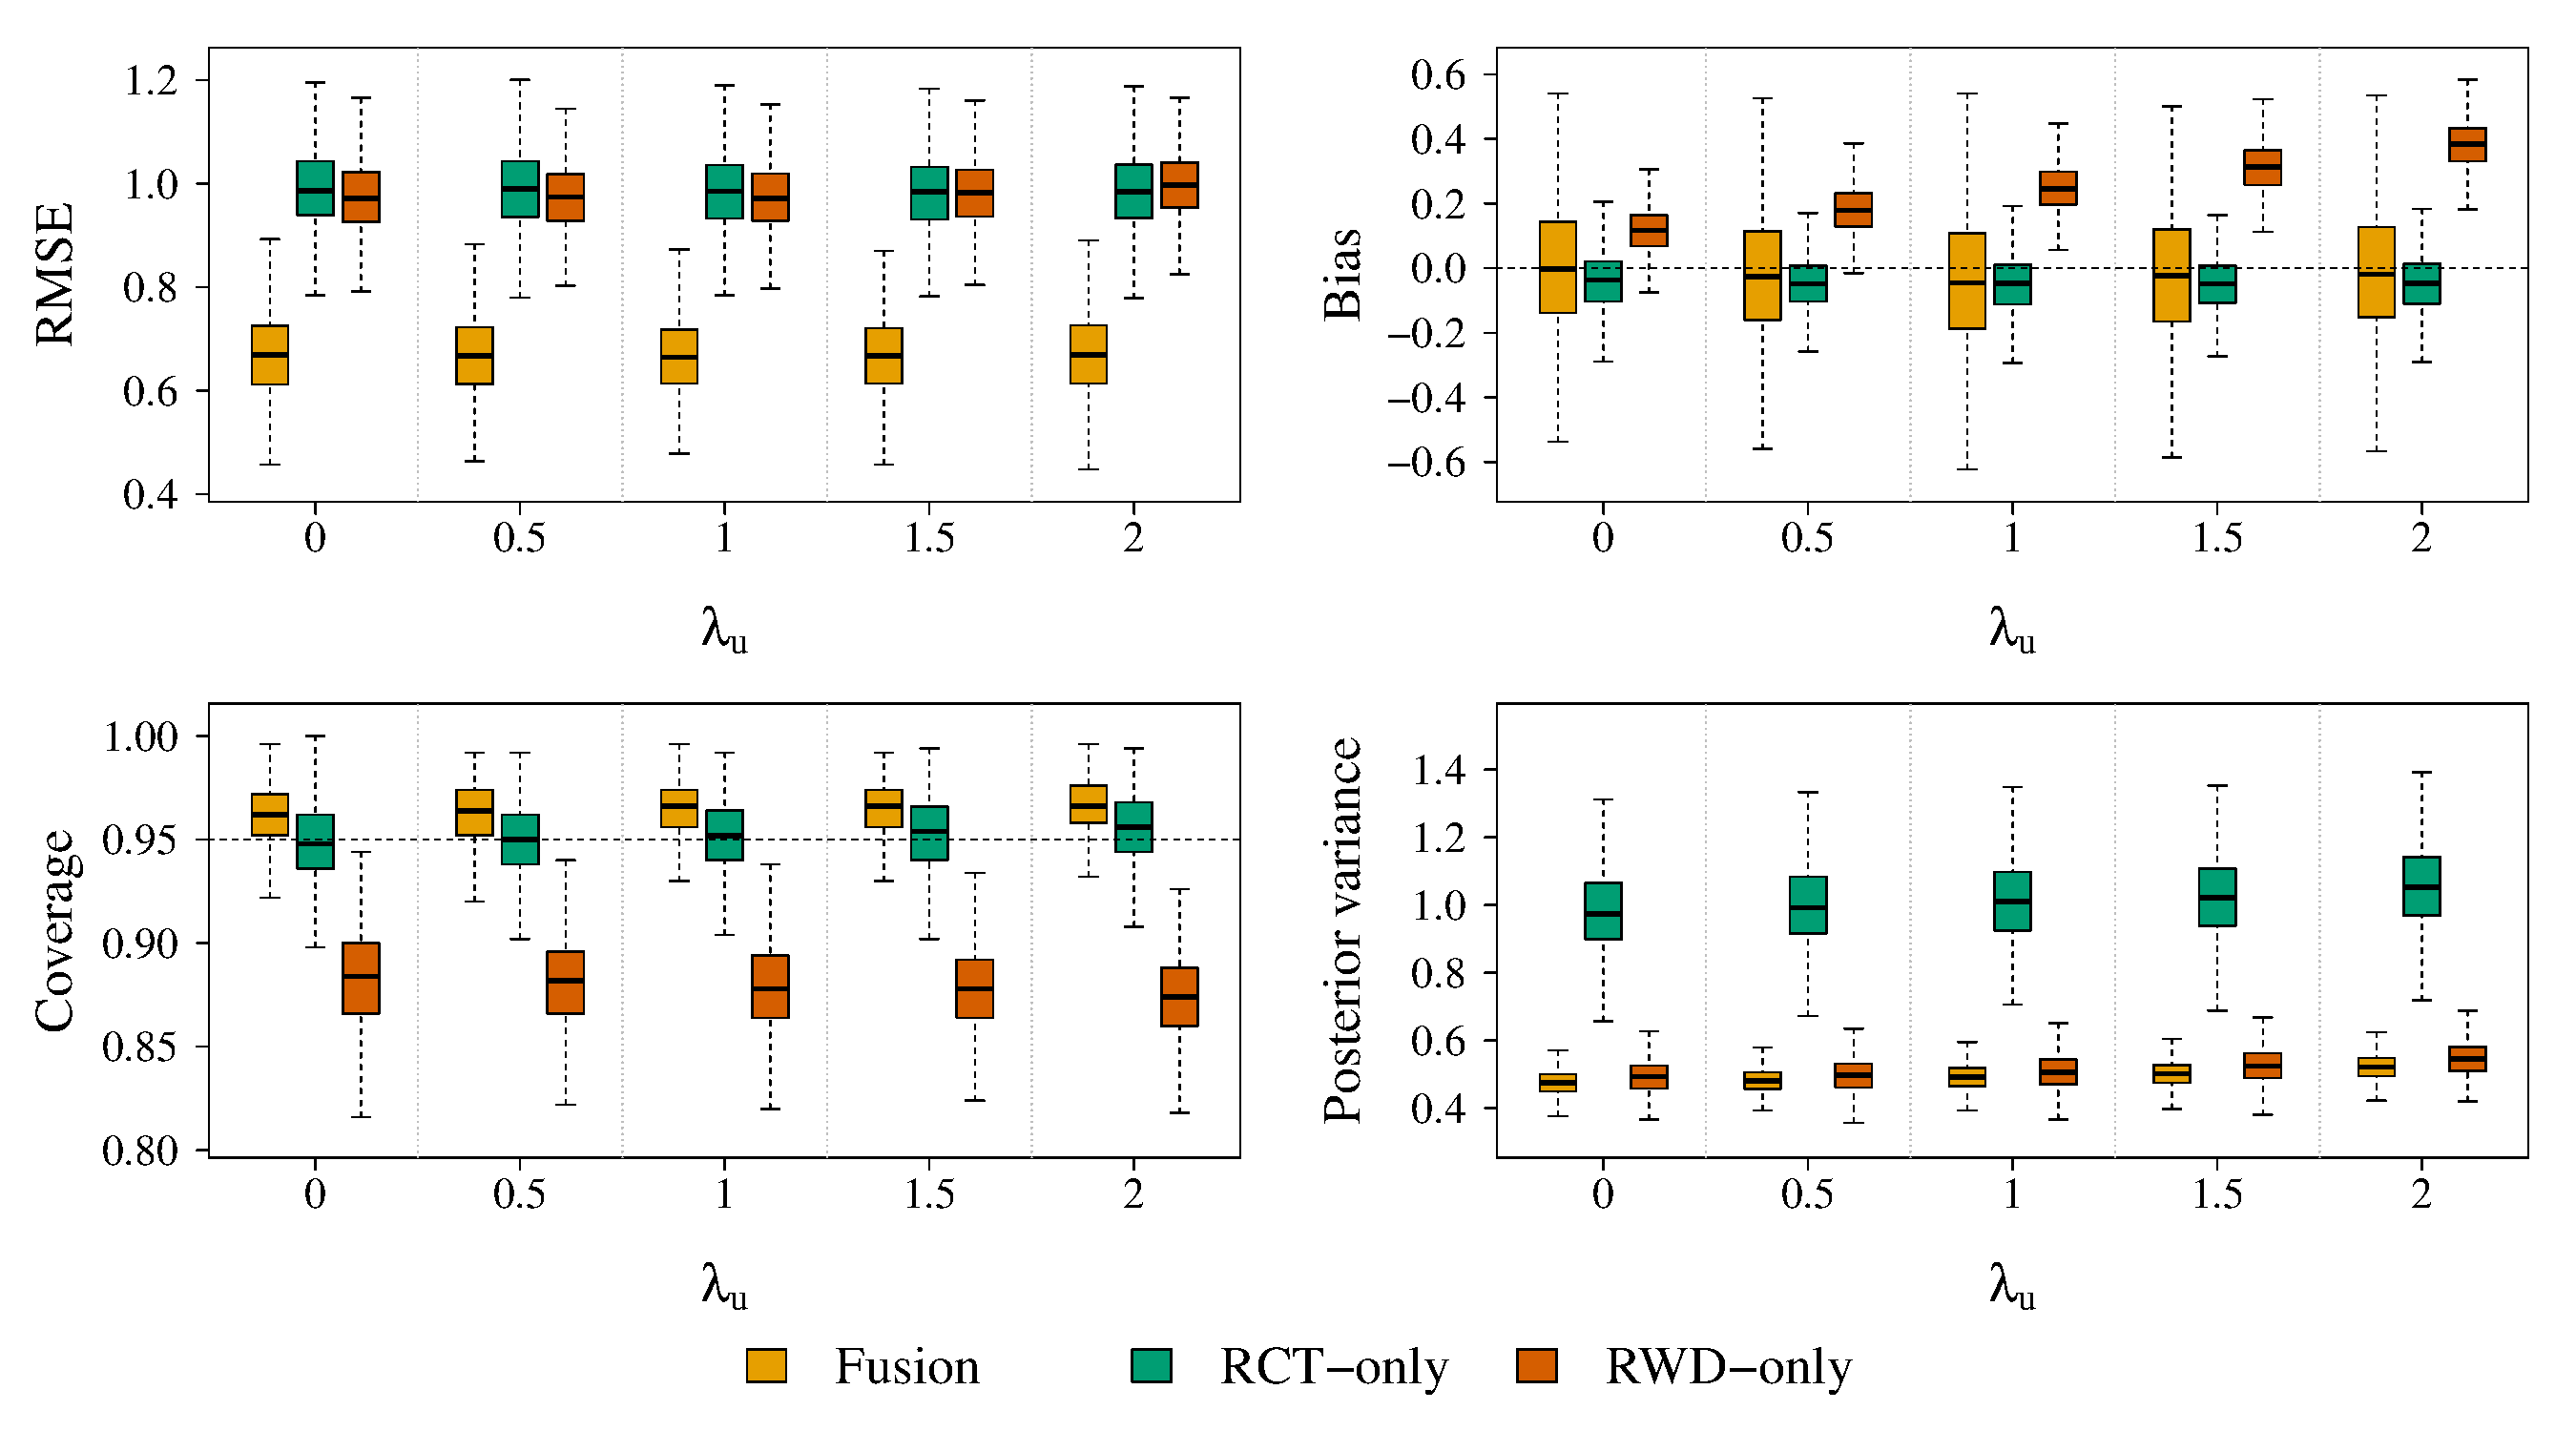
\includegraphics[width=0.8\textwidth]{sim_vary_lambda_u}
  \caption{CATE metrics under varying unmeasured confounding strength $\lambda_u$, with the RWD prognostic deviation held at $\lambda_d = 1$. From top-left to bottom-right: pointwise RMSE, mean bias, 95\% credible-interval coverage, and posterior variance of $\hat\tau(x)$, averaged over the evaluation set and across simulation replicates. Dashed reference lines indicate zero bias and nominal coverage.}
  \label{fig:sim-lambda-u}
\end{figure}

We report the results for varying between-source heterogeneity $\lambda_d$ at fixed confounding $\lambda_u = 1$ in Figure~\ref{fig:sim-lambda-d}.
All three estimators are essentially flat in $\lambda_d$.
The fusion and trial-only estimates stay unbiased and at nominal coverage.
The real-world-only estimate keeps the bias from the fixed confounding.
RMSE and posterior variance are stable across $\lambda_d$.

\begin{figure}[tb]
  \centering
  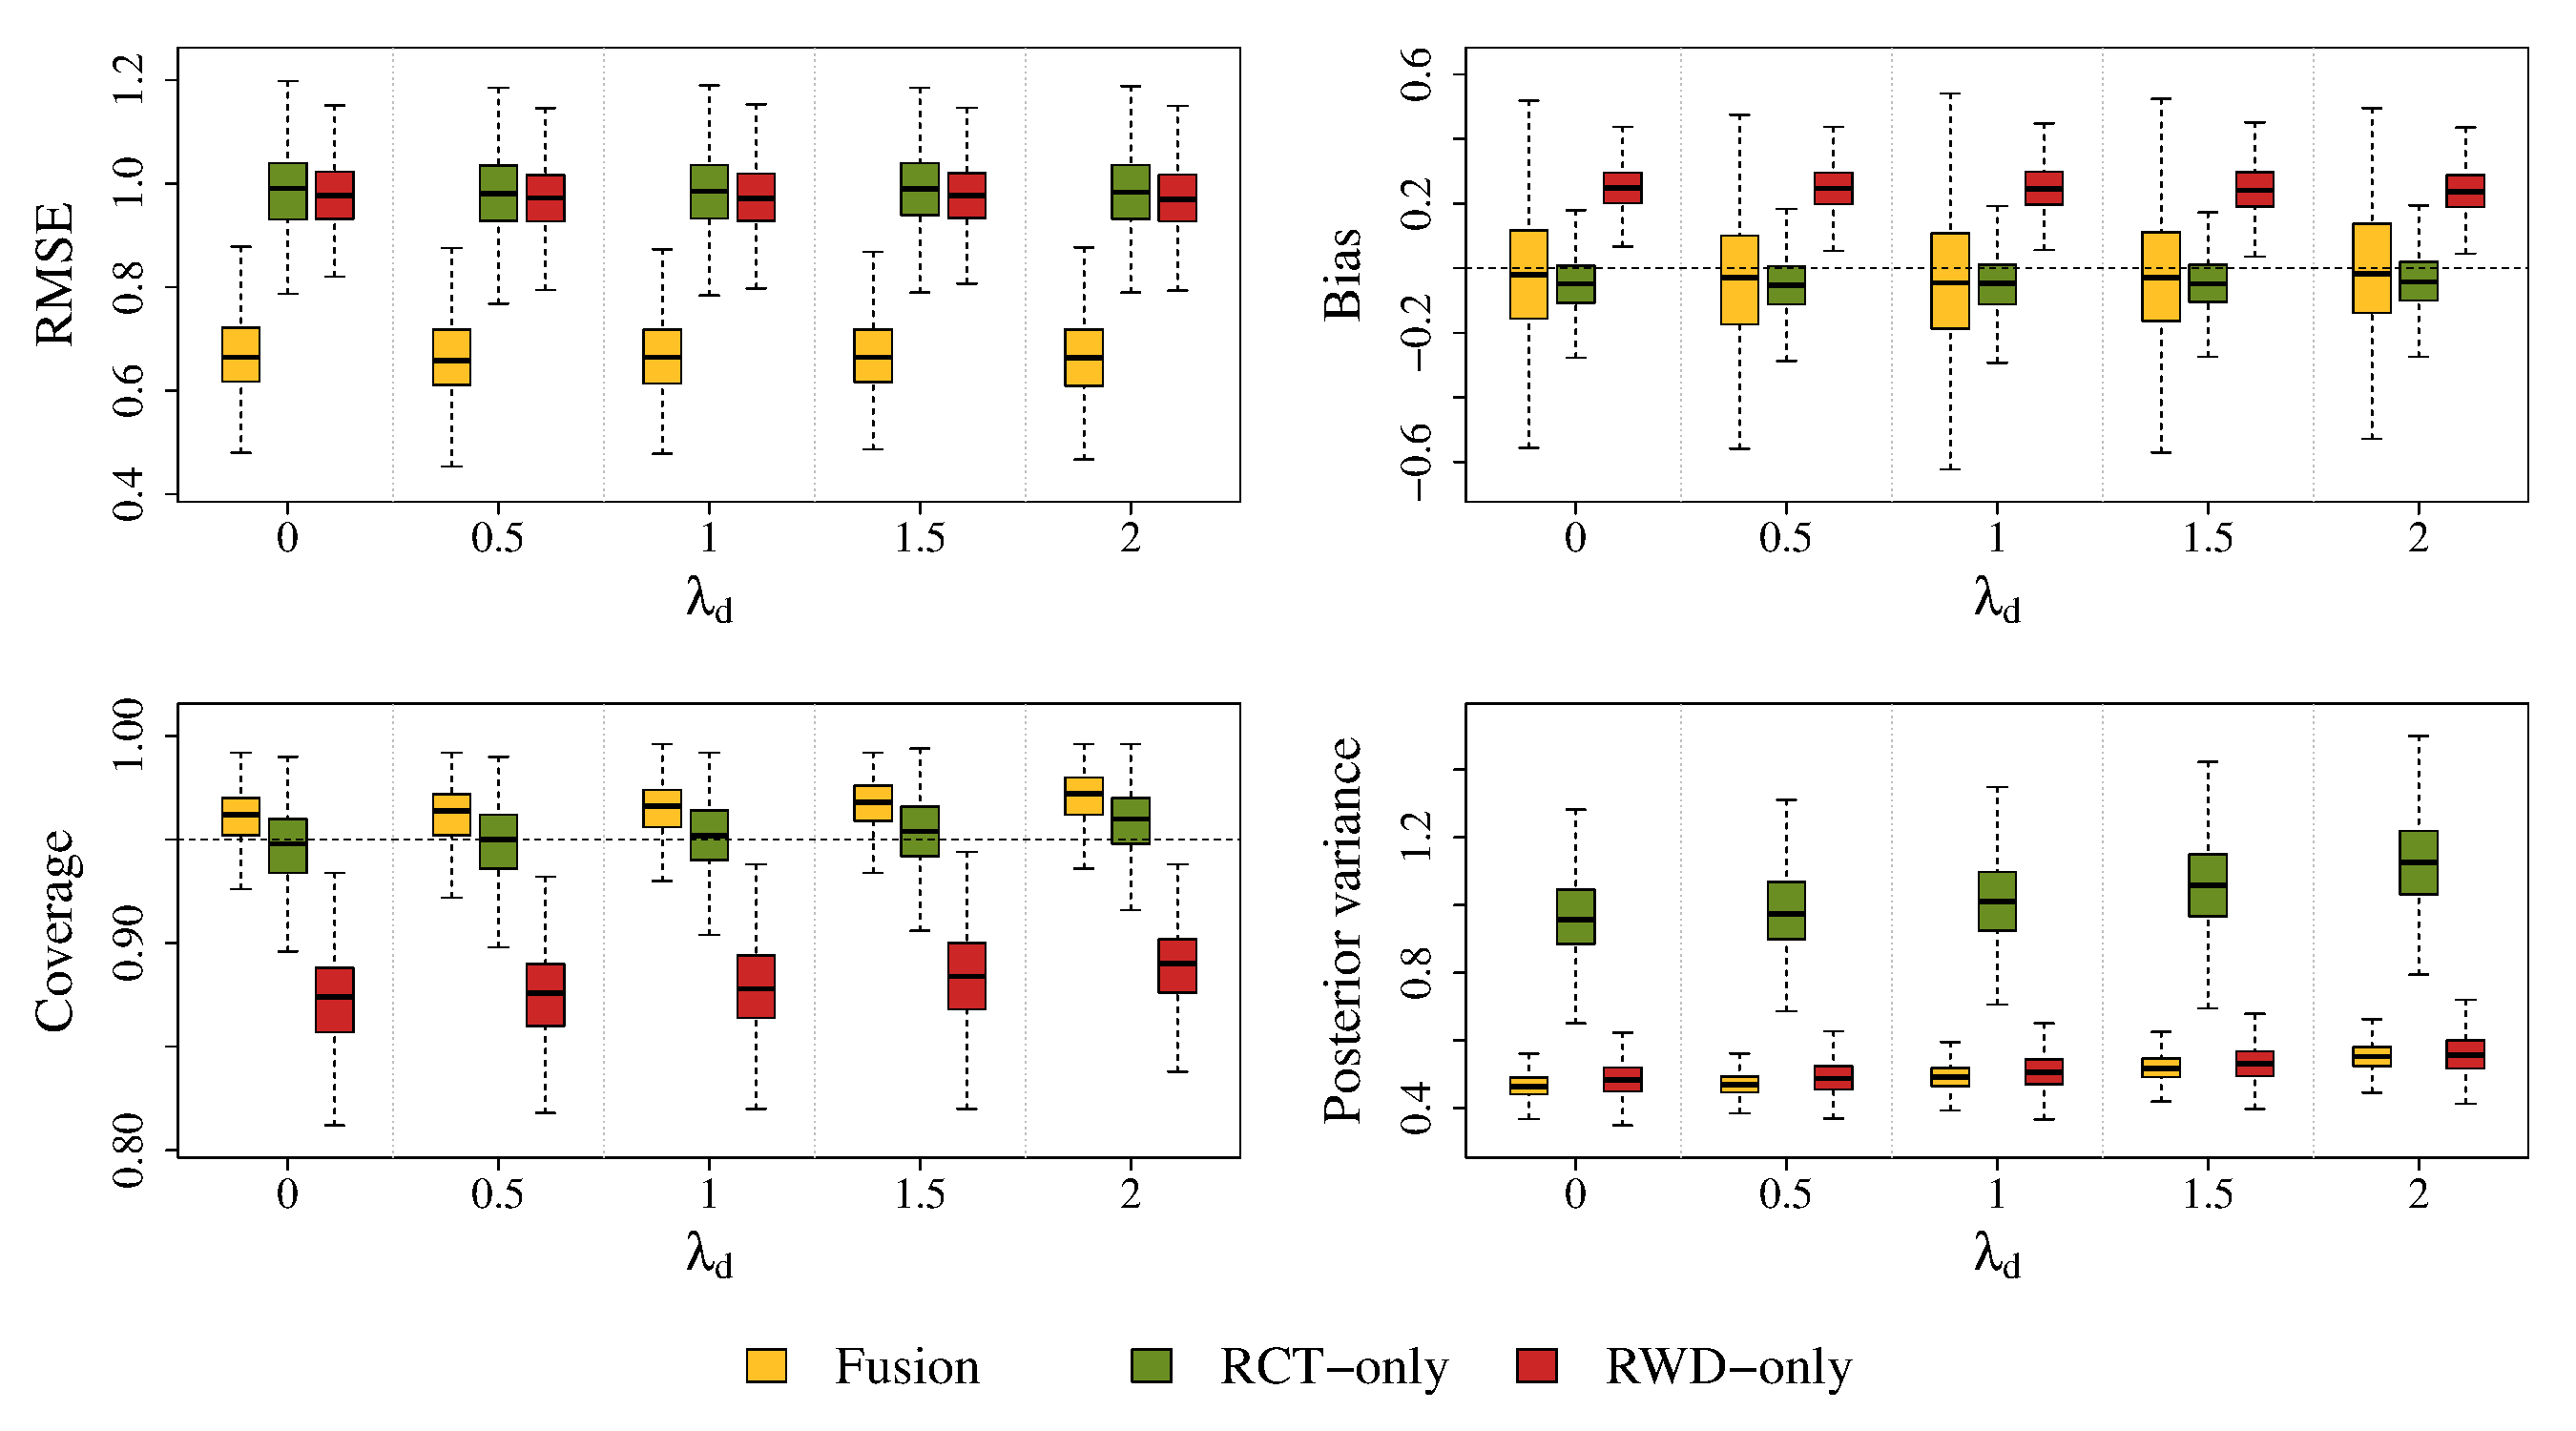
\includegraphics[width=0.8\textwidth]{sim_vary_lambda_d}
  \caption{CATE metrics under varying between-source heterogeneity $\lambda_d$, with the unmeasured confounding held at $\lambda_u = 1$. Panels, methods, and reference lines as in Figure~\ref{fig:sim-lambda-u}.}
  \label{fig:sim-lambda-d}
\end{figure}

The two experiments show that the fusion forest is robust to both nuisances.
The fusion forest corrects for the unmeasured confounding in the real-world data and stays unbiased as the confounding strengthens.
It accommodates the prognostic heterogeneity between the sources and is unaffected as the heterogeneity grows.
It also exploits the larger real-world sample and achieves lower RMSE and posterior variance than the trial-only baseline at every grid point.

% !TEX root = ../general/main.tex
\section{Application: survival after HIV}

We study the effect of a combination antiretroviral therapy versus zidovudine (ZDV) monotherapy on event-free survival in HIV.
We combine the AIDS Clinical Trials Group Protocol~175 (ACTG~175) \citep{hammer1996} with the Multicenter AIDS Cohort Study (MACS) \citep{kaslow1987}.
Treatment in ACTG~175 is randomised.
MACS is an observational cohort with unmeasured confounding \citep{hernan2000marginal}.
We pool the three combination regimens in ACTG~175 into one comparator and contrast it with ZDV monotherapy.
We restrict both sources to a common population: men with baseline CD4 count of 200 to 500 cells/mm$^3$.
This alignment makes the fusion credible, since the two sources then approximate one population \citep{pocock1976}.
We adjust for six baseline covariates: age, CD4, CD8, calendar year, race, and years of prior antiretroviral therapy.
Table~\ref{tab:cohort} summarises the aligned cohort: 1771 trial patients and 373 cohort patients.
The trial follows patients for a maximum of about three years: too short to reach median event-free survival.
The cohort follows them for about twenty-five years and reaches a median event-free survival of five to six years.
This longer follow-up adds robustness for the late treatment effect where the trial is uninformative.
MACS records outcomes at biannual visits. 
The data give event times only to the calendar year, so the events are interval-censored at annual resolution.
Figure~\ref{fig:km-curves} shows the Kaplan--Meier survival curves.

\begin{table}[b]
  \centering
  \begin{tabular}{@{}lcc@{}}
    \toprule
                                    & ACTG~175 (RCT)  & MACS (RWD)        \\
    \midrule
    Age, y                          & 34 [29, 41]     & 39 [34, 44]      \\
    CD4, cells/mm$^3$               & 337 [263, 422]  & 263 [178, 365]   \\
    CD8, cells/mm$^3$               & 918 [670, 1246] & 849 [659, 1153]  \\
    Calendar year                   & 1992            & 1991 [1991, 1992]\\
    Prior ART, y                    & 0.4 [0, 2.1]    & 1.0 [0, 1]       \\
    Non-white, $n$ (\%)             & 404 (23)        & 78 (21)          \\
    \bottomrule
  \end{tabular}
  \caption{Characteristics of the trial-aligned analysis cohort of
    $2{,}144$ patients, by data source. Continuous variables are reported
    as median [IQR], categorical variables as $n$ (\%). }
  \label{tab:cohort}
\end{table}



\begin{figure}[tb]
  \centering
  
\includegraphics[width=0.8\linewidth]{survival_curves_manuscript.pdf}
  \caption{Kaplan--Meier curves of event-free survival, by data source
    (RCT, RWD) and treatment group (ZDV monotherapy and combination).
    The main panel spans the full cohort follow-up of about 25 years;
    the inset zooms to the shorter trial window. The cohort curves are
    approximate due to interval censoring.}
  \label{fig:km-curves}
\end{figure}


We fit a Bayesian fusion forest to the combined data with default settings.
We compare it with an AFT Bayesian causal forest fitted to the trial alone.
We compute the average effect with a source-specific Bayesian bootstrap.
The source weights follow a Dirichlet prior proportional to the sample sizes.
The fusion estimate of the average acceleration factor is $1.65$ (95\% CrI: $1.43$ to $1.90$).
The trial-only baseline is close at $1.70$ (95\% CrI: $1.51$ to $1.92$).
Combination therapy stretches the event-free survival time scale by a factor of $1.65$ relative to monotherapy. 
Equivalently, the median event-free survival time under combination therapy is $1.65$ times the median under monotherapy.


The treatment effect varies across patients.
Figure~\ref{fig:cate} shows the subject-level acceleration factor for every patient, ordered by posterior mean.
The estimates lie above one, so combination helps almost everyone.
The size of the gain differs across patients.
The fusion intervals are far narrower than the trial-only intervals, which we report in the appendix.
The cohort therefore sharpens the individual estimates, not only the average.

\begin{figure}[tb]
  \centering
  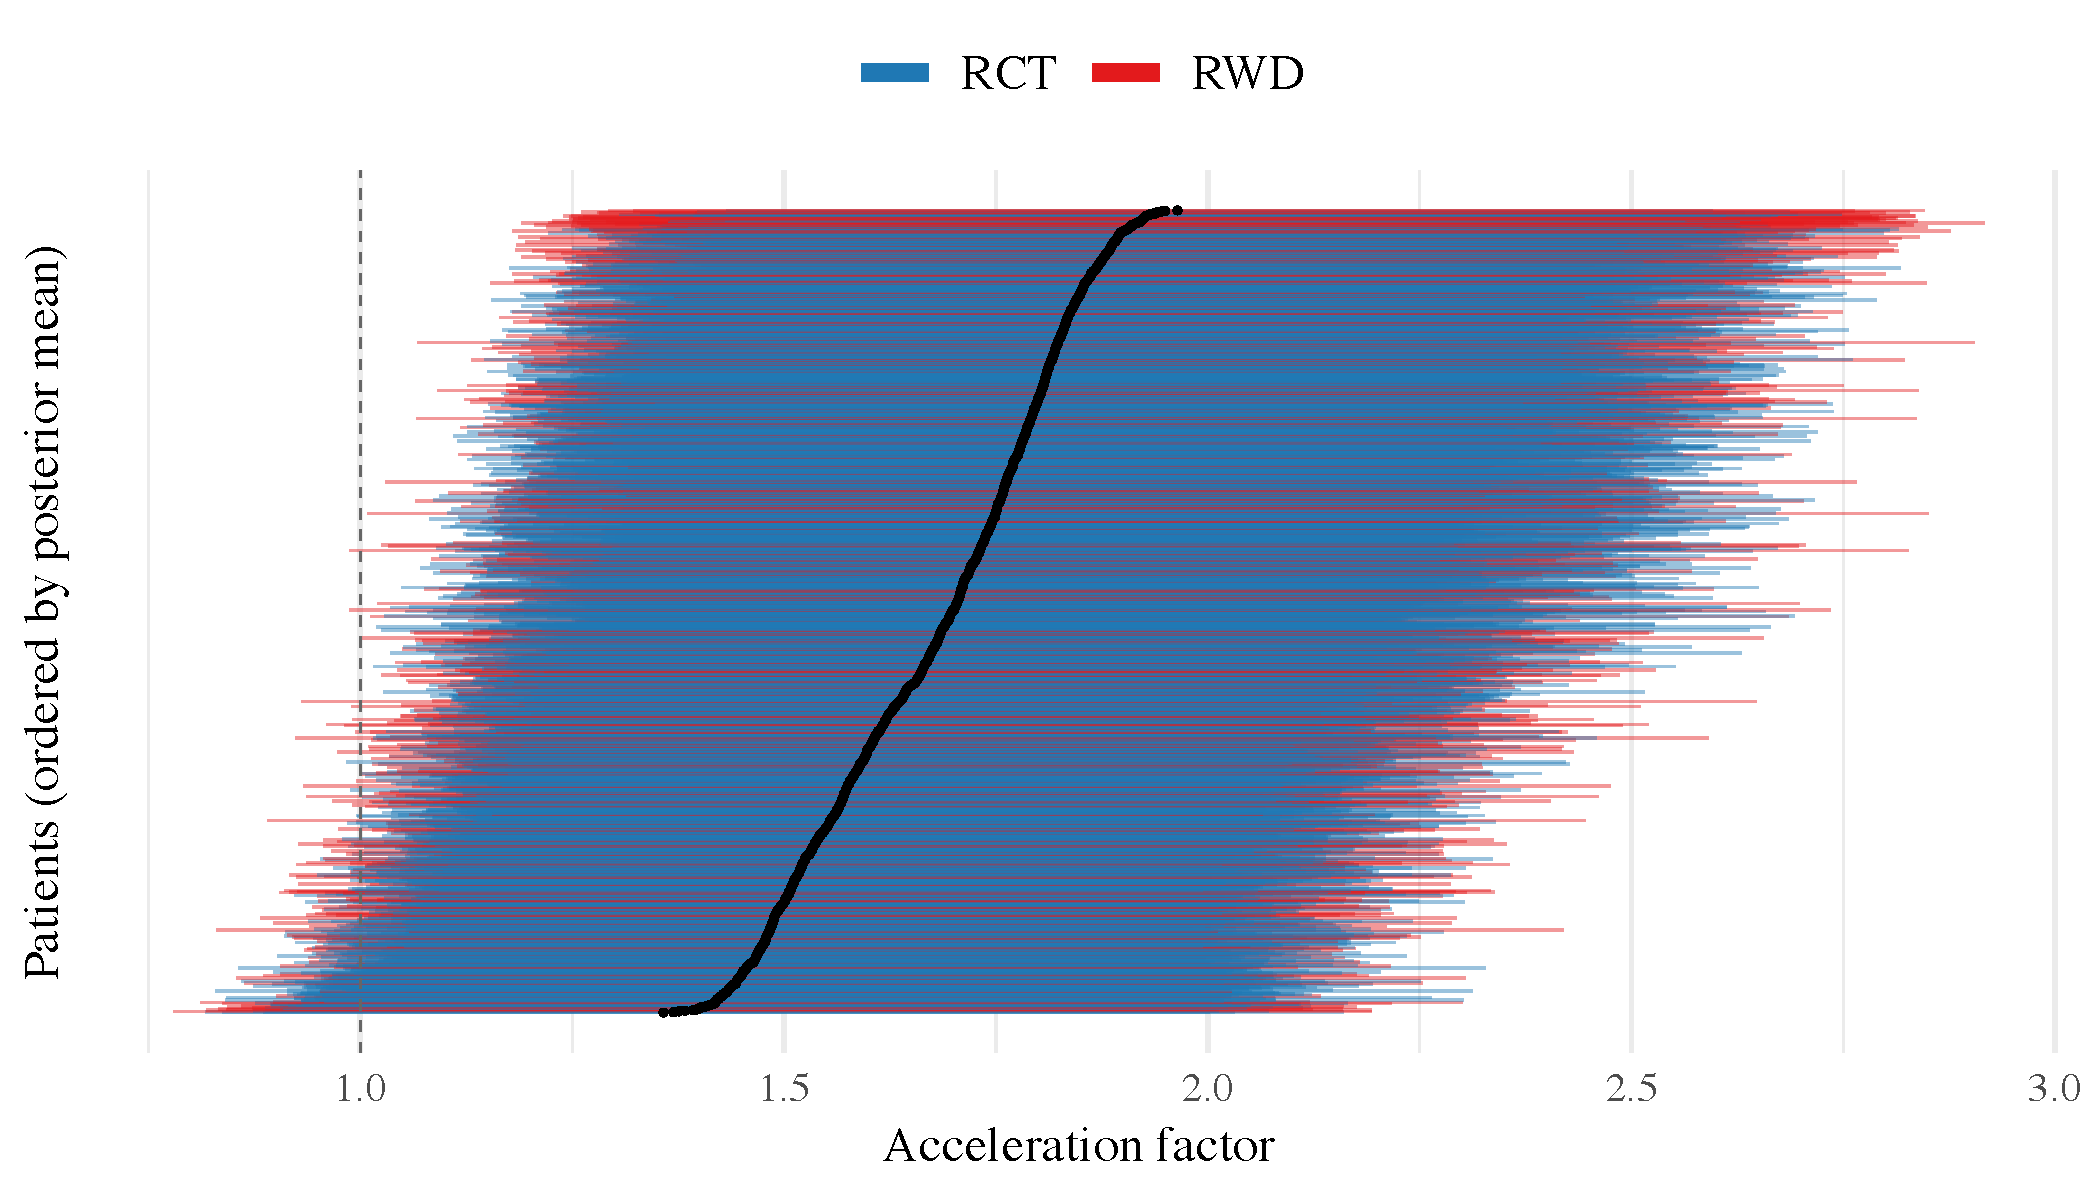
\includegraphics[width=0.8\linewidth]{cate_caterpillar_manuscript.pdf}
  \caption{Subject-level acceleration factor for every
    patient in the trial-aligned cohort, from the Bayesian fusion forest,
    ordered by posterior mean. Vertical bars are pointwise 95\%
    credible intervals; colour indicates the data source (RCT, RWD);
    the dashed line at $1$ marks no effect.}
  \label{fig:cate}
\end{figure}

We investigate how the treatment effect varies across patients. 
We use the two-stage idea behind the Virtual Twins method \citep{foster2011subgroup}.
The first stage estimates a per-patient effect, and the second fits a simple model to these estimates to locate where the effect varies.
We adapt the idea to the fusion forest as a posterior summary.
We fit the second-stage model to the posterior-mean effect and read its uncertainty from the full posterior.

We summarise the treatment effect with a regression tree (CART; \citealp{breiman1984cart}).
Figure~\ref{fig:fit-the-fit} shows a depth-three tree on the six covariates.
It splits on CD8 count and race.
The other covariates do not enter.
The acceleration factor rises with CD8, from about $1.5$ in the lowest group to about $1.8$ in the highest.
White patients gain slightly more than non-white within each CD8 band.
Every leaf exceeds $1.4$, so all subgroups benefit.
The benefit is largest at high CD8.

% Fit-the-fit summary of the FusionForest CATE.  TikZ-drawn so the
% manuscript controls the typography.  Numbers below are read off
% notes/general/figures/fit_the_fit_manuscript.pdf and matched to
% data/analysis 1/analysis_fit_the_fit.txt.
\definecolor{splitfill}{RGB}{230,244,250}
\begin{figure}[b]
  \centering
  % First arg of \resizebox is the target width -- change this fraction
  % to scale the whole figure uniformly (height auto-follows via !).
  \resizebox{0.8\textwidth}{!}{%
  \begin{tikzpicture}[
    every node/.style = {align=center, font=\footnotesize},
    splitn/.style     = {draw, rounded corners=2pt, fill=splitfill,
                         minimum width=1.15cm, minimum height=0.55cm,
                         inner sep=2.5pt},
    leafn/.style      = {draw, rounded corners=2pt, fill=white,
                         minimum width=1.45cm, minimum height=0.85cm,
                         inner sep=3pt, font=\scriptsize},
    elabel/.style     = {midway, fill=white, inner sep=4pt,
                         font=\scriptsize},
    edgeln/.style     = {draw=black!55, thick}]

    % Internal (split) nodes
    \node[splitn] (root)  at ( 0.35, 4.7) {CD8};
    \node[splitn] (mid1)  at (-3.00, 3.4) {CD8};
    \node[splitn] (mid2)  at ( 3.70, 3.4) {CD8};
    \node[splitn] (raceA) at (-4.50, 1.9) {race};
    \node[splitn] (raceB) at ( 1.70, 1.9) {race};
    \node[splitn] (raceC) at ( 5.70, 1.9) {race};

    % Leaves
    \node[leafn] (L1) at (-5.4, 0) {$1.45$\\$[1.05,\,1.92]$\\$n = 124$};
    \node[leafn] (L2) at (-3.6, 0) {$1.51$\\$[1.19,\,1.87]$\\$n = 381$};
    \node[leafn] (L3) at (-1.4, 0) {$1.60$\\$[1.31,\,1.92]$\\$n = 330$};
    \node[leafn] (L4) at ( 0.8, 0) {$1.65$\\$[1.25,\,2.13]$\\$n = 107$};
    \node[leafn] (L5) at ( 2.6, 0) {$1.72$\\$[1.43,\,2.07]$\\$n = 425$};
    \node[leafn] (L6) at ( 4.8, 0) {$1.76$\\$[1.33,\,2.32]$\\$n = 178$};
    \node[leafn] (L7) at ( 6.6, 0) {$1.83$\\$[1.51,\,2.22]$\\$n = 599$};

    % Edges
    \draw[edgeln] (root) -- (mid1)  node[elabel] {$\le 800$};
    \draw[edgeln] (root) -- (mid2)  node[elabel] {$> 800$};

    \draw[edgeln] (mid1) -- (raceA) node[elabel] {$\le 650$};
    \draw[edgeln] (mid1) -- (L3)    node[elabel] {$> 650$};
    \draw[edgeln] (mid2) -- (raceB) node[elabel] {$\le 1065$};
    \draw[edgeln] (mid2) -- (raceC) node[elabel] {$> 1065$};

    \draw[edgeln] (raceA) -- (L1) node[elabel] {non-white};
    \draw[edgeln] (raceA) -- (L2) node[elabel] {white};
    \draw[edgeln] (raceB) -- (L4) node[elabel] {non-white};
    \draw[edgeln] (raceB) -- (L5) node[elabel] {white};
    \draw[edgeln] (raceC) -- (L6) node[elabel] {non-white};
    \draw[edgeln] (raceC) -- (L7) node[elabel] {white};
  \end{tikzpicture}}
  \caption{Regression-tree summary of the acceleration factor
    $\exp\{\tau(x)\}$ from the fusion forest. We fit the tree to the
    posterior-mean log-time CATE on the six baseline covariates. Each leaf
    gives the within-leaf average acceleration factor, as a posterior mean
    and 95\% credible interval.}
  \label{fig:fit-the-fit}
\end{figure}

We inspect the posterior probability of treatment benefit $ \p(\tau(x_i) > 0 \mid \text{data})$ for each patient \citep{henderson2020individualized}.
We bin the patients by posterior probability of benefit and report the fraction in each bin.
We compute it over the trial population, under the fusion and trial-only fits, so the columns are comparable (Table~\ref{tab:hte-summary}).
We find strong evidence of benefit for almost every patient: $77\%$ have $\pi_i > 0.99$ and $97\%$ exceed $0.95$.
The trial alone is far less certain, with only $38\%$ above $0.95$ and a quarter of patients inconclusive.
The Bayesian fusion forest gains this certainty even though its average effect is slightly smaller ($1.65$ versus $1.70$).

We also summarise the between-source heterogeneity in baseline prognosis.
We fit a best-linear projection to the deviation forest  \citep{Woody2020}.
The deviation forest $d(x)$ measures how the baseline prognosis differs between the trial and the cohort.
We project $d(\cdot)$ onto the covariates by least squares.
We present the results in Table~\ref{tab:projection}.
The gap is dominated by a constant shift.
The intercept is $1.70$ (95\% CrI: $1.31$ to $2.10$), so the cohort baseline sits well above the trial.
Among the covariates, only prior antiretroviral years moves the gap, by $0.27$ (95\% CrI: $-0.01$ to $0.55$).
Age, CD4, CD8, calendar year, and race have coefficients near zero, with intervals covering zero.
The baseline prognosis therefore differs mainly through a large average shift.
This shift likely reflects population and measurement differences the six covariates do not capture.


Combination therapy prolongs event-free survival by a factor of about $1.65$.
The cohort's Kaplan--Meier curves do not reveal this benefit.
The Bayesian fusion forest recovers the effect.
The combined analysis also sharpens the individual estimates.
We identify benefit for nearly every patient, far more than the trial alone.
The treatment effect varies with CD8 count and race.
The baseline prognosis differs between the sources, through a gradient in prior antiretroviral exposure and a large average shift.

\begin{table}[tb]
  \centering
  \begin{minipage}[t]{0.46\textwidth}
    \centering
    \small
    \begin{tabular}{@{}lcc@{}}
      \toprule
      $\p(\tau(x_i) > 0 \mid \text{data})$        & Fusion & Trial-only \\
      \midrule
      $(0.99, 1]$    & $0.767$ & $0.180$ \\
      $(0.95, 0.99]$ & $0.206$ & $0.198$ \\
      $(0.75, 0.95]$ & $0.028$ & $0.364$ \\
      $(0.25, 0.75]$ & $0.000$ & $0.245$ \\
      $[0, 0.25]$    & $0.000$ & $0.014$ \\
      \bottomrule
    \end{tabular}
    \captionof{table}{Posterior probability of benefit over the trial
      population. Higher bins give stronger evidence of benefit, the
      lowest evidence of harm. Entries are fractions of patients.}
    \label{tab:hte-summary}
  \end{minipage}
  \hfill
  \begin{minipage}[t]{0.50\textwidth}
    \centering
    \small
    \begin{tabular}{@{}lcc@{}}
      \toprule
      Term          & Coefficient & 95\% CrI \\
      \midrule
      Intercept     & $1.701$  & $(1.312, 2.099)$ \\
      \midrule
      Age           & $-0.003$ & $(-0.020, 0.015)$ \\
      CD4           & $0.001$  & $(-0.001, 0.002)$ \\
      CD8           & $0.000$  & $(-0.000, 0.000)$ \\
      Calendar year & $-0.032$ & $(-0.256, 0.194)$ \\
      Race          & $0.071$  & $(-0.304, 0.443)$ \\
      Prior ART, y  & $0.269$  & $(-0.008, 0.550)$ \\
      \bottomrule
    \end{tabular}
    \captionof{table}{Best linear projection of the deviation forest
      $d(x)$ onto the covariates: posterior mean coefficient and 95\%
      credible interval on the log-transformed time scale.}
    \label{tab:projection}
  \end{minipage}
\end{table}


% !TEX root = main.tex
\section{Discussion}

We combined a randomised trial with real-world data to estimate heterogeneous treatment effects on survival outcomes, without assuming the real-world source is unconfounded.
The simulation study and the HIV application demonstrate its advantages over a single-source analysis.
The Bayesian fusion forest remains unbiased under varying levels of unmeasured confounding.
It reduces the posterior variance of a trial-only analysis.
In the application, we recovered a benefit of combination therapy that the survival curves of the real-world data alone did not reveal.
We established benefit for nearly every patient where the trial alone was inconclusive.
The model handled the right-censored trial and the interval-censored cohort jointly.

Our framework implicitly assumes the acceleration factor $\exp\{\tau(X)\}$ is time-invariant: treatment rescales the survival time by a factor that depends on the covariates but not on time.
This assumption may be inappropriate when treatment effects unfold over time, such as delayed-onset benefits or waning effects.
Flexible parametric AFT models relax this assumption by letting the acceleration factor vary with time \citep{Crowther2023}.
The causal interpretation of time-dependent acceleration factors has been formalised \citep{Brathovde2024}.
A natural extension replaces $\tau(X)$ with a generalised Bayesian tree ensemble $\tau(X, t)$.

%% The Funding, Acknowledgements and Conflict of interest sections live on the
%% title page of ../general/main.tex, because Biostatistics requires them on
%% page 1 of the manuscript. They are not repeated here. Data availability is
%% not on that page-1 list and stays here as back matter.
%%
%% Funding wording used before the Biostatistics-mandated sentence:
%%
%% This project has received funding from the European Research Council (ERC) under the European Union’s Horizon Europe program under Grant agreement No. 101074802. Views and opinions expressed are however those of the author(s) only and do not necessarily reflect those of the European Union or the European Research Council Executive Agency. Neither the European Union nor the granting authority can be held responsible for them.
%% This work used the Dutch national e-infrastructure with the support of the SURF Cooperative using grant no. EINF-18803.

%% Funding, Acknowledgements and Conflict of interest are set on the title
%% page in both main.tex (journal wording) and arxiv.tex (original ERC and
%% SURF wording), so the copies below are commented out to avoid printing
%% them twice. Data availability appears only here.
\begin{comment}
\section*{Funding}
This work was supported by the European Research Council [grant number
101074802]; and the SURF Cooperative [grant number EINF-18803].
Views and opinions expressed are those of the authors only and do not
necessarily reflect those of the European Union or the European Research
Council Executive Agency.
Neither the European Union nor the granting authority can be held responsible
for them.

\section*{Acknowledgements}
The authors used generative artificial intelligence tools in support of
developing and debugging the accompanying software.
All such output was reviewed and verified by the authors, who take full
responsibility for the content of this work.

\section*{Conflict of interest}
None declared.
\end{comment}

\section*{Data availability}
\sloppy
The software implementation is available on GitHub at \url{https://github.com/tijn-jacobs/FusionForests}.
The same repository also holds the code for the simulation studies and the data analysis.
A release on the Comprehensive R Archive Network is planned.
The ACTG~175 trial data are available in the \texttt{speff2trial} R package \citep{speff2trial}.
The MACS data can be requested through the MWCCS cohort website.

%% Flush every pending float before the references begin, so none can surface
%% inside the reference list. \FloatBarrier rather than \clearpage: it places
%% the outstanding floats without forcing a page break, so the reference list
%% starts directly under Data availability instead of on a page of its own.
\FloatBarrier
\bibliographystyle{apalike}
\bibliography{references}

\end{document}